\documentclass{article}
\usepackage{graphicx} 
\usepackage{geometry}
\geometry{left=1in, right=1in, top=1in, bottom=1in}
\usepackage{amsfonts}
\usepackage{amsmath}
\usepackage{float}
\usepackage{minted}
\title{CS 6140 Draft}
\author{qgao67 Gao}
\date{January 22th 2024}

\begin{document}
\maketitle
\section{Course 1}
\begin{itemize}
    \item \textbf{Shared memory and abstraction: }Every processor has access to every memory bank. Every processor has a memory module, which contains multiple layers and caches.
    \item We need to design the optimal network for those processors to link to each other. The goal is to minimize cost: The cost of the all-connected network is proportional to $p$, and The cost of the Interconnection network is proportional to $p^2$. The ideal network has the lowest cost.
    \item Modeling: $T = \tau + \mu * m$. $\mu$ is the inverse of network bandwidth, for example, 100Gbp/s. $\mu$ represents the cost of transmitting a single unit (0.32ns per word or 0.08ns per byte) of the message. The latency $\tau$ is close to $10^-3-10^-5$ second. If you're accessing every memory, you gonna reduce $\tau$.
    \item In a parallel communication step, each processor sends/receives one message at the same time. Suppose $P = 8$, if single communication time is  $T = \tau + \mu * m$, then all communication time is also  $T = \tau + \mu * m$ because all communications happen at the same time.
    \item A network that can route every communication at the same time can be an optimal network. For example \textbf{Benes Network: has $2*p*logp$ stages, where $p$ is the number of inputs/outputs}, Each piece of information has a unique link to send to another end. But it is completely useless in the real world because you cannot afford the time. 
    \item \textbf{Shift Permutations:} Left shift $i --- (i-1+p) \mod p$, Right shift $i --- (i+1) \mod p$.
    \item \textbf{Hypercubic Permutations:} For example: $p = 8, d = 3$. If we set j = 0, then 0=000 to 1=001, 2=010 to 3=011,... If we set j=1, then 0 to 2, 2 to 4,... If we set j=2, then 0 to 4, 2 to 6, 3 to 7...
    \item The algorithm can be good on paper, but not in practice. 
    \item We can calculate the performance matrices $p$ using $n/\tau$, where $p$ can be set $50\%$.
\end{itemize}
\section{Course 2}
\begin{itemize}
    \item How to do the task: \textbf{Finding the sum of n numbers in parallel computing:}\par
    Algorithm for $P_i$ would be:\par
    \begin{minted}{C}
    add local n/p numbers to sum
    for j = 0 to d-1 do
    if (j-th bit of rank = 1) send sum
    if ((rank AND 2^j) not equal to 0
    send sum to (rank XOR 2^j)
    else
    receive sum* from (rank XOR $2^j$)
    sum = sum + sum*
    end for
    if (rank = 0)
    print sum
      \end{minted}
\textbf{The stopping criteria is when all numbers are added to the processor where its rank equals 0, (like 000 in a $2^3$ dimensions network).}\par
      \textbf{How this adding machine works:}
      \begin{itemize}
          \item First, allocate the local summation to each processor. For example, if we have 100 numbers to add on and 10 processors, each processor calculates the sum of 100/10 numbers.
          \item The rank of each processor is represented by a binary number of $log(p)$, which is also the dimension of that hypercubic.
          \item Each processor would decide to receive or send the data based on their rank.
          Let's consider an example with 8 processors (numbered from 0 to 7), whose ranks are represented by a 3-bit binary number (since \(2^3 = 8\)). The goal is to perform a reduction operation to sum the values initially held by each processor to obtain a global sum.

In the first iteration (for \(j=0\)), we are concerned with the least significant bit (the bit corresponding to \(2^0\)). Processors will either send or receive values based on whether this bit is 0 or 1.

- \textbf{Processor 0} has a rank of 000, and its least significant bit is 0. It will not send but will receive.
- \textbf{Processor 1} has a rank of 001, and its least significant bit is 1. It will send its value to Processor 0, because \(1 \oplus 2^0 = 1 \oplus 1 = 0\).

In this case, Processor 1 sends its local sum to Processor 0. Processor 0 receives the value from Processor 1 and adds it to its own local sum.

In the second iteration (for \(j=1\)), we look at the second least significant bit (the bit corresponding to \(2^1\)).

- \textbf{Processor 2} has a rank of 010, and its second least significant bit is 1. It will send its value to Processor 0, because \(2 \oplus 2^1 = 2 \oplus 2 = 0\).
- \textbf{Processor 0} has a rank of 000, and its second least significant bit is 0. It will not send but will receive.

In this case, Processor 2 sends its local sum to Processor 0. Processor 0 now adds the value from Processor 2 to its new local sum, which already includes the values from Processors 0 and 1.

This process is repeated across all dimensions until all values are aggregated onto one processor or each processor holds a part of the global sum, depending on the final objective of the algorithm. In this way, each iteration passes some processors' local sums onto other processors, eventually achieving a global sum.
      \end{itemize}
    Visualizing the whole process would be: 
Let us consider a parallel reduction algorithm to sum the numbers from 0 to 7 using 8 processors. Each processor is initially assigned a value equal to its index. The sequence of operations is as follows:

\begin{enumerate}
    \item \textbf{Initialization}: Each processor is given an initial value:
    \begin{itemize}
        \item Processor 0 starts with value 0.
        \item Processor 1 starts with value 1.
        \item ...
        \item Processor 7 starts with value 7.
    \end{itemize}
    
    \item \textbf{1st Operation (Pairwise Summation)}: Processors perform pairwise sums in parallel:
    \begin{align*}
        \text{Processor 0} &: 0 + 1 \rightarrow \text{stores the result.} \\
        \text{Processor 2} &: 2 + 3 \rightarrow \text{stores the result.} \\
        \text{Processor 4} &: 4 + 5 \rightarrow \text{stores the result.} \\
        \text{Processor 6} &: 6 + 7 \rightarrow \text{stores the result.}
    \end{align*}
    Intermediate sums 1, 5, 9, and 13 are now stored in processors 0, 2, 4, and 6 respectively.
    
    \item \textbf{2nd Operation (Stride Summation)}: A strided sum is performed:
    \begin{align*}
        \text{Processor 0} &: \text{sum of Processor 0} + \text{sum of Processor 2} \rightarrow \text{stores the new sum.} \\
        \text{Processor 4} &: \text{sum of Processor 4} + \text{sum of Processor 6} \rightarrow \text{stores the new sum.}
    \end{align*}
    We now have two sums: 6 stored in Processor 0 and 22 stored in Processor 4.
    
    \item \textbf{3rd Operation (Final Summation)}: The final sum is computed:
    \begin{align*}
        \text{Processor 0} &: \text{sum of Processor 0} + \text{sum of Processor 4} \rightarrow \text{final sum of 28.}
    \end{align*}
    Processor 0 now holds the final result, which is the sum of numbers from 0 to 7.
\end{enumerate}

This illustrates the typical behavior of a parallel reduction algorithm, where the number of processors involved in computation reduces by half after each step, leading to \textbf{a logarithmic time complexity relative to the number of processors}, represented by $O(logN)$.\par
We consider a \textbf{parallel reduction algorithm} to sum the numbers from 0 to 7 using 8 processors, employing \textbf{XOR logic} to guide the communication between processors. Here is how the process works:

\begin{enumerate}
    \item \textbf{Initialization}: Each processor starts with a value equal to its index (ranging from 0 to 7).

    \item \textbf{1st Operation}:
    \begin{itemize}
        \item Processors focus on the least significant bit of their index (corresponding to \(2^0\)). If this bit is 0, the processor receives data; if it is 1, it sends data.
        \item For example, Processor 1 (binary 001) sends its data to Processor 0 (binary 000), as \(1 \oplus 2^0 = 0\).
        \item Similarly, Processor 3 (binary 011) sends to Processor 2 (binary 010), since \(3 \oplus 2^0 = 2\).
    \end{itemize}

    \item \textbf{2nd Operation}:
    \begin{itemize}
        \item Now, processors focus on the second least significant bit (corresponding to \(2^1\)). Processors send or receive data in strides of 2.
        \item For instance, Processor 2 (binary 010) sends its data (which includes the sum of Processors 2 and 3) to Processor 0 (binary 000), as \(2 \oplus 2^1 = 0\).
        \item Similarly, Processor 6 (binary 110) sends to Processor 4 (binary 100), since \(6 \oplus 2^1 = 4\).
    \end{itemize}

    \item \textbf{Subsequent Operations}:
    \begin{itemize}
        \item In subsequent steps, processors continue to perform XOR operations based on different bits to determine the targets for sending and receiving.
        \item The number of participating processors halves with each operation, as each operation combines the data of two processors.
    \end{itemize}

    \item \textbf{Final Result}:
    \begin{itemize}
        \item After a sufficient number of steps, all data is eventually combined into a single processor, which holds the sum of numbers from 0 to 7.
    \end{itemize}
\end{enumerate}

This XOR-based approach allows processors to effectively pass data between them, eventually achieving the aggregation of all values. The efficiency of this method lies in its ability to reduce data in logarithmic time complexity, which is highly beneficial for large-scale parallel computing.

\item Message Passing Interface\par
The standard for parallel programming via message passing.
\item Communicators: mpiexec -np 4 ./p2
\item Coding: longer than one week, 3 projects
\end{itemize}
\section{Course 3 }
\begin{itemize}
    \item \begin{minted}{C}
    int MPI_Send(void* buf, int count,
    MPI_Datatype datatype, int dest, int tag, MPI_Comm comm);
    int MPI_Recv(void* buf, int count,
    MPI_Datatype datatype, int source, int tag, MPI_Comm comm, MPI_Status* status);
    \end{minted}
    \item Message envelope contains: source rank (int src); destination rank (int dest); tag (integer used to distinguish messages); Communicator (universe of communication, MPI comm)
\end{itemize}
\section{Course 4 Prefix Sum}
\begin{itemize}
    \item Prefix Sums Problem
Input $n$ numbers: $x_0, x_1, x_2, \cdots, x_{n-1}$

Output: $S_0, S_1, S_2, \cdots, S_{n-1}$
$$
S_i=\sum_{j=0}^i x_j
$$
\item Best sequential algorithm
$$
\text { - } T(n, 1)=\Theta(n)
$$
$$
\begin{array}{|l}
S_0=x_0 \\
\text { for } i=1 \text { to } n-1 \\
S_i=S_{i-1}+x_i
\end{array}
$$
This means that \textbf{in calculating the sequential sum problem, the time complexity $T(n,1)$ (n numbers and 1 process per time) is linearly proportional to n as n increases.} (using big O notion $\theta$)\par
A simple codes shown with Jupyter Ntbook:
\begin{figure}[H]
    \centering
    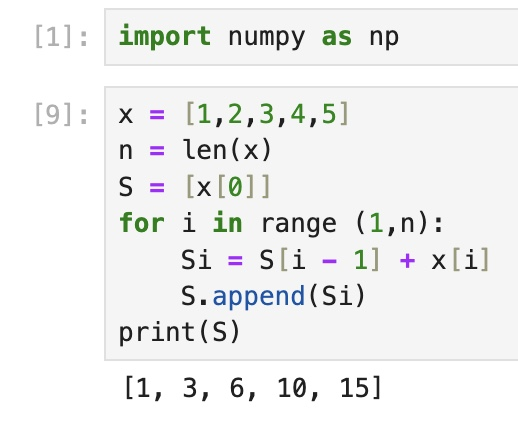
\includegraphics[width=0.5\linewidth]{Image 1-31-24 at 10.38.jpeg}
    
    
\end{figure}
\end{itemize}
\end{document}